\taskpic{ Во всех точках кривой $A$, изображённой на рисунке,
  потенциал электрического поля, созданного неподвижными точечными
  зарядами $q_1$ и $q_2$, равен $\phi$. Определите расстояние $l$
  между зарядами.}  
{
  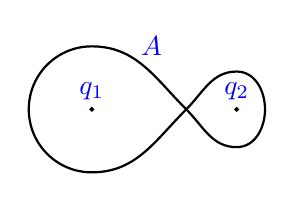
\begin{tikzpicture}[scale=0.8]
    \draw[fill=black] (1,2) circle (0.03cm) node[blue,above] {$q_1$};
    \draw[fill=black] (3.3,2) circle (0.03cm) node[blue,above] {$q_2$};
    \draw[thick] (0,2) to[out=90,in=180] (1,3) to[out=0,in=135]
    (2.5,2) to[out=-45,in=180] (3.3,1.4) to[out=0,in=-90] (3.75,2)
    to[out=90,in=0] (3.3,2.6) to[out=180,in=45] (2.5,2) to[out=225,in=0]
    (1,1) to[out=180,in=270] (0,2);
    \draw (1.95,3) node[blue] {$A$};
  \end{tikzpicture}
}
